Ein LC-Schwingkreis besteht aus einer Spule mit der Induktivität $L$ und einem Kondensator mit der Kapazität $C$. Die Spule speichert ein magnetisches Feld und der Kondensator ein elektrisches. In dem Schwingkreis wechseln sich beide Felder periodisch ab mit der Folge, dass sich der Stromfluss  mit gleicher Periode umkehrt. Zwei LC-Schwingkreise können durch einen weiteren Kondensator $C_\text{K}$ gekoppelt werden (siehe Abbildung \ref{fig:Abb2}). \\
\begin{figure}[h!]
	\centering
	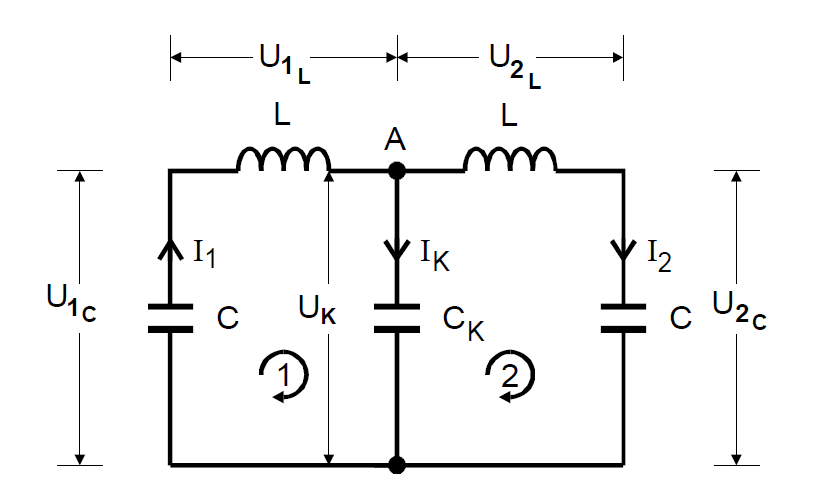
\includegraphics[width=0.7\textwidth]{Abb2.png}
	\caption{Gekoppelter LC-Schwingkreis}
	\label{fig:Abb2}
\end{figure}
Der Stromfluss in beiden einzelnen gekoppelten Kreisen wird durch die Kirchhoffschen Regeln bestimmt.
\begin{align}
I_\text{K} = I_\text{1}-I_\text{2} \\
U_\text{1C} + U_\text{1L} + U_\text{K} = 0 \\
U_\text{2C} + U_\text{2L} + U_\text{K} = 0
\end{align}
Die gekoppelten Differentialgleichungen für beide Schwingkreise folgen mit
\begin{align}
U_\text{C} = \frac{1}{C} \int I \dd t \quad \text{und} \quad U_\text{L} = L \dv{I}{x} \quad .  \\
\text{1. DGL:} \quad L \dv[2]{I_1}{x} + \frac{1}{C} I_1 + \frac{1}{C_\text{K}}(I_1 + I_2) = 0 \\
\text{2. DGL:} \quad L \dv[2]{I_2}{x} + \frac{1}{C} I_2 - \frac{1}{C_\text{K}} (I_1 + I_2) = 0
\end{align}
Durch entkoppeln der Differentialgleichungen folgen Lösungen für die einzelnen Ströme $I_1$ und $I_2$ mit den Frequenzen $\nu+$ und $\nu^-$. Die Lösungen sind zudem abhängig von den Anfangsamplituden $I_{10}$ des erstem Schwingkreises und $I_{20}$ des zweiten Schwingkreises.
\begin{align}
I_1(t) = \frac{1}{2}(I_{10} + I_{20}) \cos(2 \pi \nu^+ t) + \frac{1}{2}(I_{10} - I_{20}) \cos(2 \pi \nu^- t) \\
I_2(t) = \frac{1}{2}(I_{10} + I_{20}) \cos(2 \pi \nu^+ t) - \frac{1}{2}(I_{10} - I_{20}) \cos(2 \pi \nu^- t)
\end{align}
Die Frequenzen sind
\begin{align}
\nu^+ = \frac{1}{2 \pi \sqrt{L C}} \quad \text{und} \label{Frequenz_p} \\
\nu^- = \frac{1}{2 \pi \sqrt{L\left(\frac{1}{C} + \frac{2}{C_\text{K}}\right)^{-1}}} \quad . \label{Frequenz_m}
\end{align}
Nun werden wichtige Spezialfälle dieses komplexen Verhaltens beschrieben. Die zwei \textbf{Fundamentalschwingungen} zeichnen sich dadurch aus, dass die Anfangsamplituden $I_{10}$ und $I_{20}$ gleich groß sind ($\abs{I_{10}} = \abs{I_{20}}$). Sind beide Schwingkreis in Phase ($I_{10}=I_{20}$) schwingen sie mit der Frequenz $\nu+$. Der Koppelkondensator hat hier keine Funktion. Er ist zu keinem Zeitpunkt geladen. Der Schwingkreis verhält sich wie ein einfacher LC-Kreis. Sind die Schwingkreise um eine halbe Periode phasenverschoben ($I_{10} = - I_{20}$) schwingen sie mit der etwas höheren Frequenz $\nu-$. Die höhere Frequenz entsteht dadurch, dass der Koppelkondensator einem periodisch wechselnden Stomfluss ausgesetzt ist und den normalen Kondensator unterstützt. \\
Das Phänomen der \textbf{Schwebung} tritt auf, wenn einer der Kreise stimuliert wird bzw. eine Anfangsamplitude hat und der andere Kreis keine Anfangsamplitude aufweist. Beim Aufstellen der Gleichungen wird ausgenutzt, dass die Frequenzen $\nu^+$ und $\nu^-$ nahezu übereinstimmen. \\

\todo{Ich finde du wiederholst dich hier, wenn du sagst, dass die Frequenzen nahezu übereinstimmen.}
\todo[color=green]{Findest du es so besser?}

\begin{align}\label{Schwebung}
	I_1(t) = I_{10}  \cos \left( \pi (\nu^+ + \nu^-) t \right) \cdot  \cos \left( \pi (\nu^+ - \nu^-) t \right) \\
	I_2 (t) = I_{10}  \sin \left( \pi (\nu^+ + \nu^-) t \right) \cdot  \sin \left( \pi (\nu^+ - \nu^-) t \right) 
\end{align}
Es entsteht eine Schwingung (siehe Abbildung \ref{fig:Abb3})  mit den Frequenzen der einzelnen Schwingkreisen 
\begin{equation}
	\nu = \pi (\nu^+ + \nu^-)
\end{equation}
und einer Schwebungsfrequenz von 
\todo[inline]{Ich glaube hier müsste ein Minus sein und die 2 weg.}
\todo[inline, color = green] {Das Minus muss auf jeden Fall hin, bei der zwei bin ich mir ziemlich sicher. Das hatten wir auch im Koloquium besprochen. In der Anleitung steht vor der anderen Formel halt ein 1/2.}
\begin{equation}
	f = 2 \pi (\nu^+ - \nu^-) \quad .
\end{equation}
Es handelt sich um einen periodischen Energieaustausch zwischen den beiden Schwingkreisen mit der Schwebungsfrequenz.
 \begin{figure}[h!]
 	\centering
 	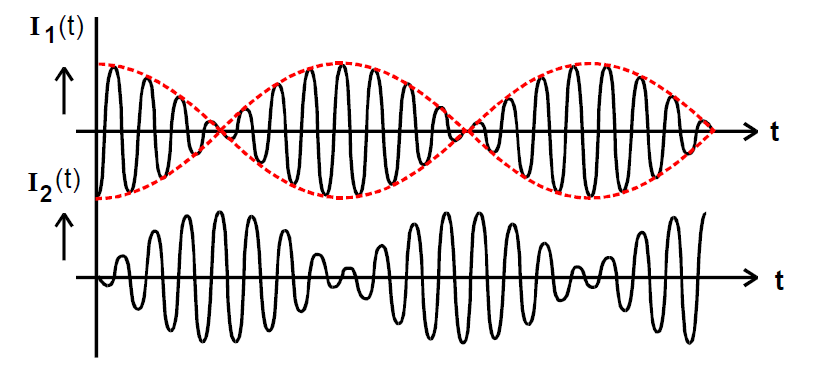
\includegraphics[width=0.7\textwidth]{Abb3.png}
 	\caption{Stromveräufe beider Schwingkreise im Fall der Schwebung}
 	\label{fig:Abb3}
 \end{figure}